% % % % % % % % % % % % % % % % % Preamble for notes % % % % % % % % % % % % % % % % % % % % % % % %
\documentclass[12pt,oneside,a4paper]{article}


% % % % % Sprogpakker og Layout % % % % % % % % %
\usepackage[left=2.5cm,top=2.0cm,bottom=1.8cm, right=2.5cm]{geometry}
%\usepackage{ulem}
\usepackage[danish,english]{babel}
\usepackage[utf8]{inputenc}
\linespread{1.3}       % simulerer Word 1.5 line spacing


% % % % % % % % % % Øvrige vigtige pakker % % % % %
\usepackage[font={small,sl},labelfont={bf, up}]{caption}
\DeclareCaptionLabelFormat{subfig}{\figurename #1~\arabic{figure}\alph{subfigure}:}
\captionsetup[subfigure]{labelformat=subfig}
\usepackage{graphicx}
\graphicspath{{./Figures/}}
\usepackage{amsmath}
\usepackage{amssymb}
\usepackage{url}
\usepackage{psfrag}
\usepackage{cancel}
\usepackage{booktabs}
\usepackage{pdfpages}
%\usepackage{mathpazo}
\usepackage[section]{placeins}
\usepackage{wrapfig}
\usepackage{tocloft}
\usepackage{subcaption}
\usepackage{epstopdf}
\usepackage[separate-uncertainty = true]{siunitx}
\usepackage{fancyhdr}
\usepackage{pageslts}
%Muliggør 'flere figurer i én' Eksempel på anvendelse (indenfor figure-environment):
% \subfloat[undercaption 1]{\label{label 1}\includegraphics[bredde 1]{billede 1}}
% \subfloat[undercaption 2]{\label{label 2}\includegraphics[bredde 2]{billede 2}}
% \caption{overordnetcaption}
% \label{overordnet label}
\usepackage{lscape}
%Omdanner en del af dokumentet til landscape. Angives med \begin{landscape}
\usepackage{framed}
%Sætter en ramme om et område begrænset af \begin{framed} og \end{framed}.
%Allows footnotes
\usepackage{footnote}
\setlength{\parindent}{0cm}
\setlength{\parskip}{0.3cm}
% % % % % % COMMANDS % % % % % % % %

\numberwithin{equation}{section}

\begin{document}

\selectlanguage{english}
% % % % % % % % % % % % % % % % % % % % % % Forside % % % % % % % % % % % % % % % % % % % % % % % % %
\pagenumbering{roman}

\begin{center}
{\textsc {\LARGE \bf{Københavns Universitet \\[0.3cm]  Bachelorstudiet i fysik}}}\\[1.5cm]
{\textsc {\Large \bf Førsteårsprojekt 2017}}\\[0.8cm]
{\Large Projekt nummer: 2017-06}\\[1cm]

\rule{15cm}{0.01cm}\\[1cm]
{\LARGE\bf  Bouncing ball}\\ [0.5cm]
\rule{15cm}{0.01cm}\\[1cm]
\end{center}

\vfill
{\large Forfattere:}\\
{\large \hspace*{1cm} \makebox[6cm][l]{Andreas M. Faber}  \hspace{1cm} KU- ID: \makebox[2cm][l]{QZJ517} \\
{\large \hspace*{1cm} \makebox[6cm][l]{Benjamin T. Søgaard}   \hspace{1cm} KU- ID: \makebox[2cm][l]{MGX877} \\
{\large \hspace*{1cm} \makebox[6cm][l]{Joachim J. Kønigslieb}   \hspace{1cm} KU- ID: \makebox[2cm][l]{GWC666} \\

{\large Vejledere:}\\
{\large \hspace*{1cm} \makebox[6cm][l]{Jörg Helge Müller}  \hspace{1cm} Email: \makebox[2cm][l]{muller@nbi.ku.dk} \\

\vfill

{\large Rapporten omfatter {\bf \lastpages{arabic}{1}} siders 
hovedtekst og 
{\bf 
\lastpages{roman}{2}} siders appendix.}

{\large Rapporten er indsendt som en pdf-fil den 17. marts 2017. }

\normalsize


% % % % % % % % % % % % % % % % % % % % % % Abstract  og Indholdsfortegnelse % % % % % % % % % % % % % % % % 
\newpage
\selectlanguage{danish}
\begin{abstract}
\setlength{\parindent}{0cm}
\setlength{\parskip}{0.3cm}
\noindent I denne opgave vil vi undersøge den kaotiske opførsel af et system 
bestående af en  kugle hoppende på en vibrerende højtaler membran. For at 
beskrive systemet introducerer vi grundlæggende begreber i kaosteori ved at 
undersøge den logistiske afbildning. Samtidig beskriver vi Feigenbaums 
$\delta$, som er en vigtig konstant for periode doblende fænomener. For at 
analysere systemet opstiller vi en teoretisk model, som vi løser med numeriske 
metoder. Simulationen viser sig at opføre sig som forventet og giver et ret 
præcist estimat af Feigenbaums $\delta$.

Da vi lavede eksperimentet fandt vi dog at vores idealiserede model af højtaleren ikke passede særlig godt med virkeligheden, hvilket resulterede i nogle store forskelle mellem vores teoretiske model og vores eksperimentelle data. Dog kunne vi stadig give et rimeligt bud på Feigenbaums $\delta$ gennem vores data.


\end{abstract}

\selectlanguage{english}
\begin{abstract}
\setlength{\parindent}{0cm}
\setlength{\parskip}{0.3cm}
\noindent In this report we will investigate the chaotic behaviour of a ball 
bouncing on a vibrating loudspeaker membrane. In doing this, we describe 
fundamental principles of chaos theory by examining the simple case of the 
logistic map. We also introduce the Feigenbaum $\delta$, which is an almost 
universal constant for dynamical systems that exhibit period doubling such as 
the logistic map and the bouncing ball. To examine the system we created a 
theoretical model, which we solved using numerical methods. The simulation 
conformed beautifully to the theory of period doubling phenomena, and gave us a 
quite accurate estimate of Feigenbaums $\delta$.

However, when we conducted the actual experiment we found that the ideal loudspeaker used in our model represented the one in the experiment quite poorly. The result of this was we could not properly fit our model to our experimental data. Despite this, we were still able to give a quite reasonable estimate of Feigenbaums $\delta$ through our experimental data.
\end{abstract}

\newpage

\tableofcontents


% % % % % % % % % % % % % % % % % % % % % % Indhold % % % % % % % % % % % % % % % % % % % % % % % % %
\newpage
\pagenumbering{arabic}
\section{Introduction to chaos}
\label{chaos}
We will soon see that our experiment exhibits chaotic behaviour. In physics, 
chaotic behaviour is often defined as a dynamical system so sensitive to 
initial conditions that its behaviour becomes impossible to predict after a 
certain amount of time, since unmeasurable differences in initial conditions 
lead to drastically different outcomes. In other words, two arbitrarily close 
initial conditions can make the system evolve into two states arbitrarily far 
apart. This is of course a rather loose definition, and it can therefore be 
useful to take a moment to examine a simpler chaotic system which has many of 
the same qualities our experiment has.

\subsection{The Logistic Map \& Cobweb Diagrams}

Consider the simple non-linear recurrence relation
\begin{equation}
x_{n+1}=\lambda x_n (1-x_n)
\label{logmap}
\end{equation}
This is called the logistic map, and it has some very interesting properties. However, in this paper we will only examine these qualitatively, since the logistic map is only presented to get some familiarity with behaviour that arises from our experiment. First of all, we will want to consider only cases where $0<x_0<1$ and $0<\lambda<4$, since outside this restriction the series quickly diverges to $-\infty$. Within these restrictions, we can graphically iterate \eqref{logmap} by plotting the functions $f(x)=\lambda x_n (1-x_n)$ and $g(x)=x$. First, we start off with an $x_0$ and draw a vertical line until we intersect $f(x)$. The coordinates of this point are now $(x_0,x_1)$. To find $x_2$, we need to find$x_1$ on the $x$-axis, such that we can plug it into $f(x)$ to obtain $x_2$. Therefor, we go horizontally to $g(x)$ to obtain the coordinates $(x_1,x_1)$, and we can now return to $f(x)$ vertically to find $(x_1,x_2)$, and so on. Two examples with different initial conditions ($x_0$) but same $\lambda$ can be seen on figures \ref{cobx1l20} and \ref{cobx8l20}

\begin{figure}
	\centering
	\begin{subfigure}{0.45\textwidth}
		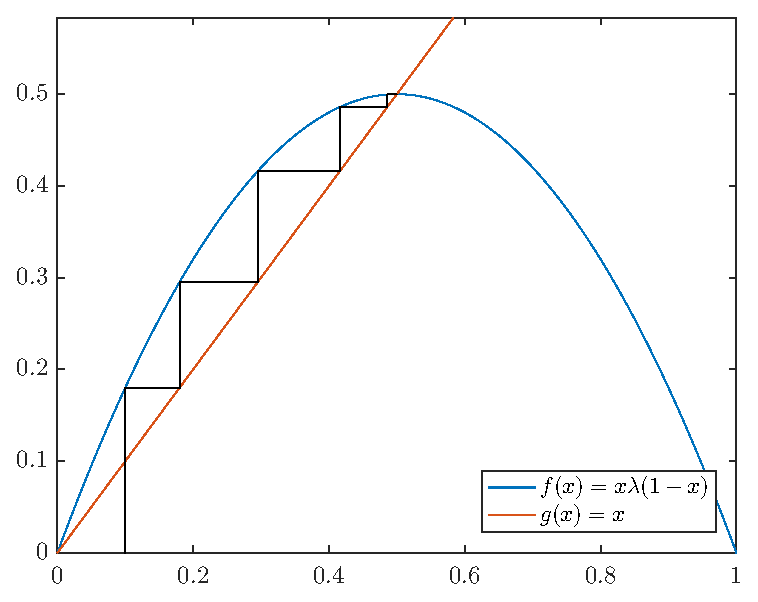
\includegraphics[width=\linewidth]{cobweb_x1_l20_iter50}
		\caption{Cobweb diagram with $x_0=0.1$ and $\lambda=2$}
		\label{cobx1l20}
	\end{subfigure}\hfill
	\begin{subfigure}{.45\textwidth}
	\centering
			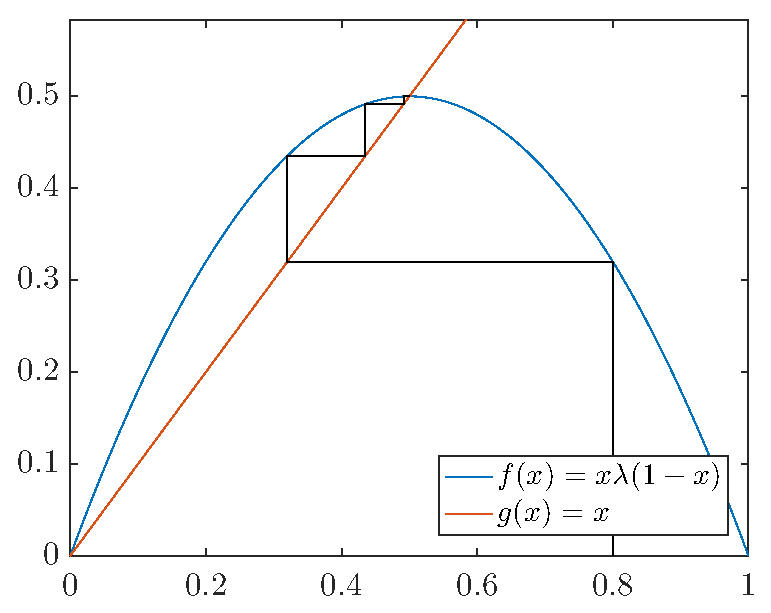
\includegraphics[width=\linewidth]{cobweb_x8_l20_iter50}
	\caption{Cobweb diagram with $x_0=0.8$ and $\lambda=2$}
	\label{cobx8l20}
\end{subfigure}
\end{figure}

If we play around with different values for $\lambda$ and 
$x_0$, we quickly see that while $\lambda<3$, the series converges to the 
intersection between $f(x)$ and $g(x)$. Since this point is determined only by our choice of $\lambda$ 
and not $x_0$, the series converges to the same value regardless of our initial conditions. The point
the series converges to is called an attractor, and it is a common behavior in non-linear dynamical
systems for there to be some point or set of points that attracts regions of initial conditions. For this particular system, something remarkable happens to this attractor if we permit $\lambda>3$.

\subsection{Bifurcation Diagrams \& Feigenbaums $\delta$}
For $\lambda$ slightly greater than 3, $x_n$ is no longer attracted to a single 
value, but rather starts bouncing between two distinct values as $n \rightarrow 
\infty$. For $\lambda$ even greater, $x_n$ will bounce between 4 values, then 8 
and so on\footnote{cobweb diagrams of this behavior can be found in appendix 
\ref{cobwebapen}}. When the attractor splits like this, we call it a 
bifurcation, and it happens infinitely many times as we let $\lambda$ increase 
from 3 to 4. To try to get a better overview of this behavior, we can create 
what is called a bifurcation diagram. In this diagram, we sweep through 
different values of $\lambda$ and see where $x_n$ ends up. An example of this 
with $2.75<\lambda<4$ can be seen on figure \ref{bifurcation}.
\begin{figure}
	\centering
	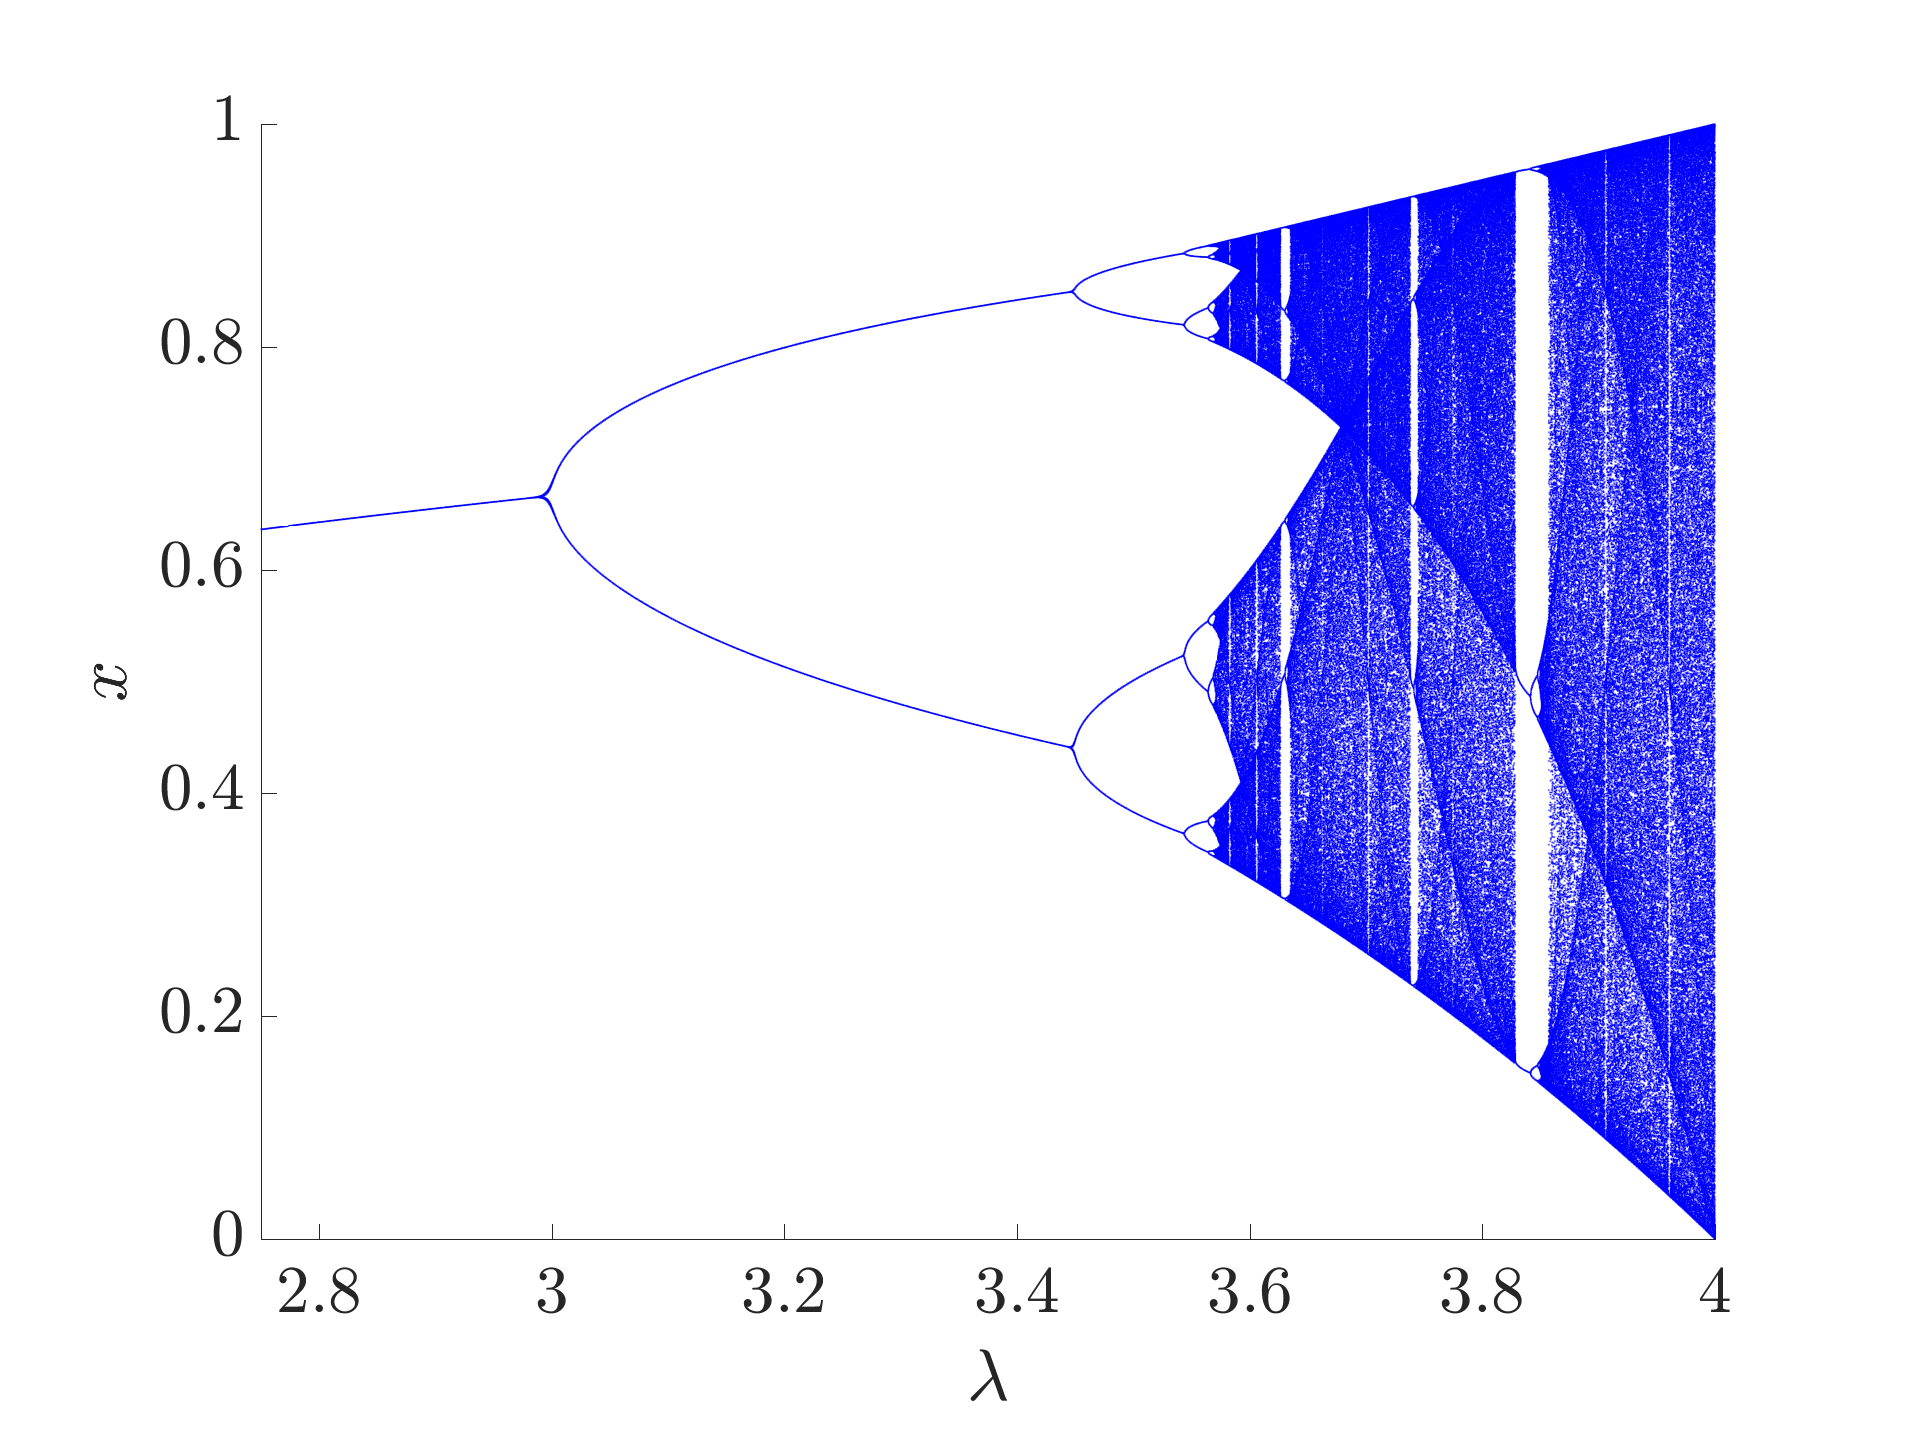
\includegraphics[width=0.65\linewidth]{Figures/Bifurcation}
	\caption{Bifurcation diagram of the logistic map for $2.75<\lambda<4$}
	\label{bifurcation}
\end{figure}
On the $x$-axis we have our different values of $\lambda$, and on the $y$-axis we plot the last 128 values of $x_n$ after 500 iterations. The key to understanding the bifurcation map is that we have 128 values of $x_n$ for each $\lambda$, which is of course what allows us to see the bifurcations. This diagram clearly allows us to see the first couple of bifurcations, but at some point it seems like the plot just degenerates into chaos. The reason for this, is that the distance between each bifurcation decreases approximately geometrical, so the infinitely many bifurcation occur in a finite range of $\lambda$s. On the plot it very quickly becomes difficult to distinguish between 128 distinct different values of $x_n$, or pure chaos. However, as we continue to increase $\lambda$, we see islands where order reemerges from the chaos, and the attractor briefly consists of 3 values, after which it splits to 6 and so on. It actually turns out that for any given number, there exists a region where the attractor consists of that many points somewhere in the diagram. How quickly after one another these bifurcations come can be approximated with something called Feigenbaums $\delta$ \cite{strogatz}. Mitchell Feigenbaum found out that as the number of bifurcations increase, the ratio between the distance between two consecutive bifurcations converges to a constant given by
\begin{equation}
\delta=\lim_{n \to \infty} \frac{\lambda_{n-2} - \lambda_{n-1}}{\lambda_{n-1}-\lambda_n} \approx 4.67 \label{Feigenbaumsdelta}
\end{equation}
Feigenbaum proved that this value converges, and that it does so rather quickly, which is important, because it means that it can be approximated rather reasonably with just the first 3 bifurcations. It amazingly also turns out that this constant holds (approximately) true for many other chaotic dynamical systems that display bifurcating nature, one of these systems being our bouncing ball. This is why we will give our estimate of Feigenbaums $\delta$ later, through both our simulation and experimental data.
\section{Model of the system}
\label{modelling}
\subsection{Experimental setup}
We have placed a small steel ball on top of a concave glass lens on glued to a vibrating speaker membrane, as depicted on figure \ref{sketch}. This set-up traps the ball in an up-and-down motion governed by the parameters of the loudspeaker vibration. Placing the system on a hard stone floor, we try to eliminate any resonance effects between the system and the outside world. By placing 4 layers of translucent scotch tape on the lens we reduce to coefficient of restitution. This reduces the chances of the ball doing any horizontal movement in the pit of the lens, or jumping out of the lens altogether. 
\begin{figure}[h]
	\centering
	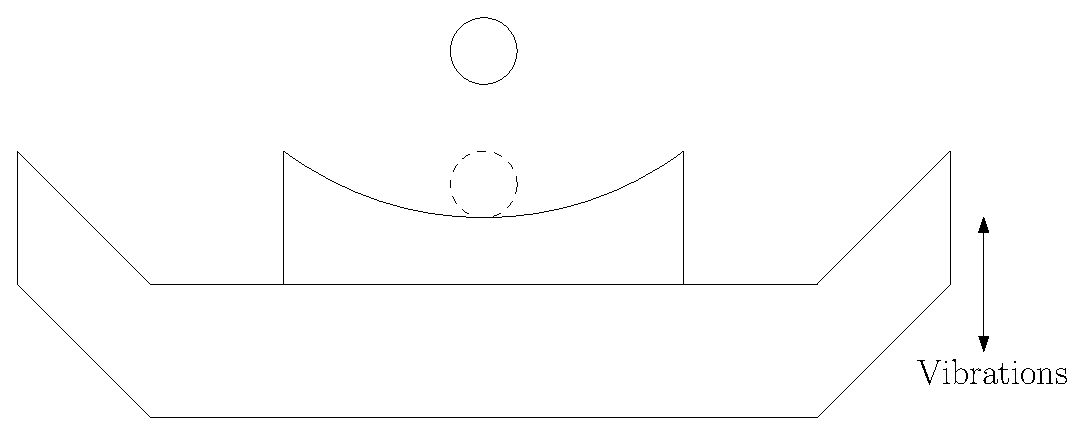
\includegraphics[width=0.55\textwidth]{speaker2}
	\caption{Sketch of the setup with the described loudspeaker and concave lens.}
	\label{sketch}
\end{figure}
\subsection{General model}
We will model our experiment as a 1-dimensional system, which is to say we will not 
account for sideways motion. On figure \ref{bounces} two consecutive bounces 
can be seen where the latter is higher due to the speaker membrane moving upwards at the 
time of impact.
\begin{figure}[h]
	\centering
	\includegraphics[width=0.65\textwidth]{Figures/bounceplot.eps}
	\caption{Plot of two bounces on the vibrating membrane}
	\label{bounces}
\end{figure}
The $k^{\text{th}}$ bounce can be completely described by the time $t_k$ it left the membrane and the velocity $v_k$ at that instance. Time and phases $\phi_k$ can be used interchangeably through the relationship $\phi=2\pi f t$.

To describe the system during a specific bounce we denote the distance of the 
ball above the rest position of the membrane $y_b(t)$. Similarly we define 
$y_p(t)$ as the displacement from equilibrium. For a given frequency $f$, phase 
shift $\phi$ and amplitude $A$ the equation of motion for the membrane is
\begin{equation}
	y_p(t)= A \cos(2\pi f t+ \phi)
	\label{membraney}
\end{equation}
In the air the ball is essentially a body in free fall, and since it is quite small and dense, the air resistance can be ignored. Thus the equation of motion for the ball $y_b(t)$ for the $k^\text{th}$ jump, with the initial conditions $v_k$, $y_p(t_k)$ at time $t_k$, is simply given by
\begin{equation}
	y_{b,k}(t) = -\frac{g}{2}(t-t_k)^2+v_k(t-t_k)+y_p(t_k)
	\label{ybeq}
\end{equation}
For each jump we will denote the change of the impact $y$-coordinate\footnote{In general it is not possible to find $\Delta y_k$ analytically as it would require one to find the intersection between the graph of a parabola and a sine wave.} as $\Delta y_{k}=y_p(t_{k+1})-y_p(t_{k})$. Plugging that into (\ref{ybeq}) and solving for $t$ determines the flight time of each jump.
\begin{equation}
	\Delta t_{k} = t_{k+1}-t_{k} = \frac{v_{k}+\sqrt{v_k^2-2g\Delta y_k}}{g}
	\label{flytime}
\end{equation}
Furthermore we can differentiate equation (\ref{ybeq}) to find the velocity of the ball, thereby finding the final velocity for each jump $v_{k,f}$.
\begin{equation}
	v_{b,k}(t) = -g(t-t_k)+v_k \Rightarrow v_{k,f} = v_{b,k}(t_k+\Delta t_k) = 
	-\sqrt{v_k^2-2g\Delta y_k}
\end{equation}
To model the impact between the ball and the membrane we use a constant 
coefficient of restitution $C_r$ although more complex models have been 
suggested\cite{muller}. For a membrane at rest, the velocity after the impact 
is proportional to the velocity before by $C_r$ such that $v_{up}=-C_r 
v_{down}$. For a moving membrane we simply transform into the coordinate system 
where the membrane is at rest, calculate the velocity of the ball in this frame 
and then transform back. The velocity of the membrane is easily obtained by 
differentiating (\ref{membraney}).
\begin{equation}
	v_p(t) = 2\pi f A \sin(2\pi f t+ \phi)
	\label{membranev}
\end{equation}
Putting the two together yields the following relationship between the final velocity of the $k^{th}$ jump $v_{k,f}$ and the initial velocity of the next $v_{k+1}$.
\begin{align}
	v_{k+1} &= -C_r(v_{k,f}-v_p(t_k+\Delta t_k))+v_p(t_k+\Delta t_k) \nonumber \\
	&= C_r \sqrt{v_k^2-2g\Delta y_k}+2(C_r+1)\pi f A \sin(2\pi f (t_k+\Delta t_k)+ \phi) \label{impactv}
\end{align}
Equation (\ref{impactv}) looks quite complicated as it is for the most general case, but as we shall see in the next section it can be simplified through a number of assumptions.

\subsection{Period-1 stable orbit}
If we consider the most simple stable state of our system, it is when the ball is bouncing with identical trajectories. A more formal way of stating this, is that $\Delta t_k$ should be constant. By  (\ref{flytime}) this would further imply that the initial velocity $v_k$ is the same for every bounce. For this to be true we must assume the phase at the impact also remain constant e.g. $\Delta y_k=0$. Which leads to the conclusion that the flight time must equal a whole number full period $\Delta t_k = \frac{n}{f}$ with $n\in \mathbb{N}$. Taking advantage of this fact together with (\ref{flytime}) yields the initial velocity for each jump
\begin{equation}
	\Delta t_k = \frac{n}{f} = \frac{2v_k}{g} \Rightarrow v_k = \frac{ng}{2f}
	\label{1perv}
\end{equation}
Denoting the phase of impact by $\theta$ we can simplify (\ref{impactv}).
\begin{equation}
	v_{k+1} = C_rv_k+2(C_r+1)\pi fA \sin(\theta)
\end{equation}
Substituting (\ref{1perv}) into the expression and solving for $\theta$ gives
\begin{align}
	\frac{ng}{2f} = C_r\frac{ng}{2f}+2(C_r+1)\pi fA \sin(\theta) \Rightarrow \sin(\theta) = \frac{ng}{4\pi Af^2 }\frac{C_r-1}{C_r+1}
	\label{1perstable}
\end{align}
The first thing to notice about (\ref{1perstable}) is that it does not have a solution for all parameter sets. That is not all selections of amplitude and frequency can sustain a bouncing motion, as they do not provide a sufficient amount of energy to balance the loss due to the impact. Since $\sin: \mathbb{R} \rightarrow [-1,1]$, we can determine when \eqref{1perstable} has a solution. The upper bound can be  ignored since the right hand side is clearly always negative, as $C_r<1$.
\begin{align}
	-1 \le \frac{ng}{4\pi Af^2 }\frac{C_r-1}{C_r+1} \Rightarrow \sqrt{\frac{ng}{4\pi A}\frac{1-C_r}{C_r+1}} \le f
\end{align}
The above result is interesting in the sense that it is the lower frequency 
limit for a sustained bouncing motion. By differentiating (\ref{membranev}) 
again we can determine the minimum frequency for the ball to experience 
momentarily weightlessness is $f\ge\sqrt{\frac{g}{4\pi^2A}}$, the ratio between 
the two is
\begin{equation}
	r_f=\frac{\sqrt{\frac{g}{4\pi^2A}}}{\sqrt{\frac{ng}{4\pi A}\frac{1-C_r}{C_r+1}}} = \sqrt{\frac{1}{n\pi} \frac{1+C_r}{1-C_1}}
\end{equation}
We use a set-up with $C_r\approx 0.7$ and $n=1$ which gives $r_f\approx1.3$. 
This means that the ball can get into a stable 1-period before the vibrating 
membrane can self-start it. It should be noted that the lower bound is greater 
in practice since the theoretical lower bound indicates when there is exactly 
enough energy in the system for a stable period. It is not however hard to 
provide the precise initial conditions to reach a stable period at such low 
frequencies, as one would have to produce matching phase and velocity 
conditions. When $r_f$ is below unity, the system will keep restarting the ball 
without outside interaction, allowing the attractor to take over. Also this 
theoretical analysis suggests that a stable 1-period exists for all parameter 
sets that satisfy the above equation. In practice this is not true however, 
since the ball is much more likely to slip into a higher numbered period at 
higher frequency. 
\section{The experiment}
\label{expsetup}
\subsection{Schematic of the experimental setup}
The setup used for the experiment can be seen on figure \ref{setupdia}. In 
essence the setup allows us to control a function generator through a PC as 
well as collect data about the impacts with the ball. The operation is as 
follows: We set a desired frequency and amplitude on the PC (6), which 
communicates this information to the micro controller (5) through USB. The 
micro controller outputs a digital sine wave from a table to a DAC at constant 
amplitude. A separate DAC is used to amplify the signal from the first DAC. 
This is done to prevent loss of resolution at low amplitudes. The analog signal 
is then routed on to the amplifier (7), which can output a signal ranging from 
\SI{+15}{V} to \SI{-15}{V} as provided by the power supply (8). The amplifier 
is connected to the actual loudspeaker (2), which then vibrates at the 
desired parameter set.
\begin{figure}[h]
	\centering
	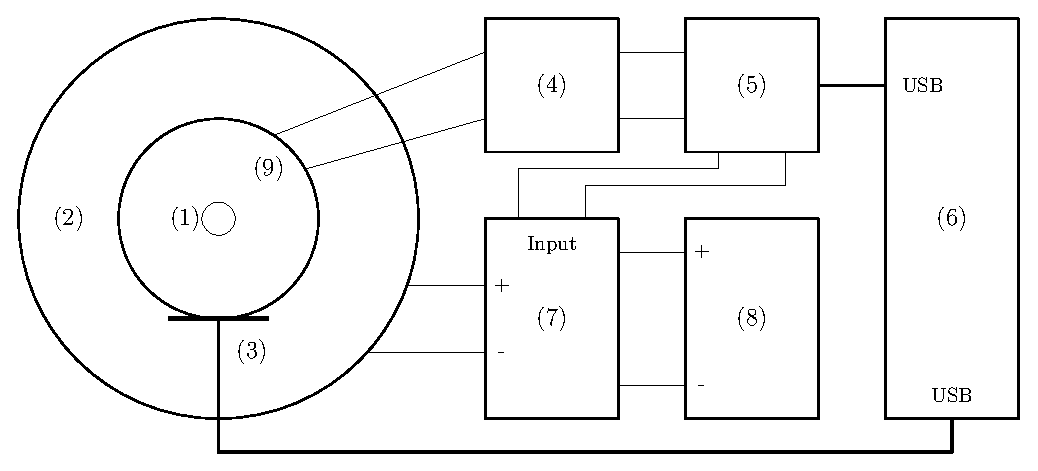
\includegraphics[width=0.8\textwidth]{setup}
	\caption{Schematic of the setup: (1) Steel ball, (2) loudspeaker with concave lens, (3) Accelerometer attached to the lens, (4) Filter and trigger circuit, (5) Micro controller and DACs, (6) PC, (7) Amplifier, (8) Power supply, (9) Piezoelectric element}
	\label{setupdia}
\end{figure}
As the ball (1) starts to bounce on the concave lens, which was chosen to 
minimize sideways motion, the piezoelectric element (9) induces a voltage when 
the ball impacts. The piezoelectric element is connected to a small circuit (4) 
that partly consists of a low pass filter and partly of a adjustable reference 
voltage to change the emphasis of the signal. Lastly the filtered signal is 
passed on to the micro controller which acts as a comparator and thereby 
determine whether there has been an impact or not. For every impact the micro 
controller sends back relevant information about the impact, such as phase, to 
the PC.

In the following section \ref{Characterization} we will examine how well the 
set-up can deliver the desired parameter set. To do this we attached an 
accelerometer (3) to the loud speaker giving us vital data about the waveform 
such as frequency, amplitude and phase shift.
\subsection{Characterization of the setup}
\label{Characterization}
To perform the experiment we wish the parameters of the speaker membrane to be independent of each other. That is, amplitude should not depend on frequency, the 'sine-lyness' of the produced waveform should not depend on amplitude etc. As it turned out, this was not always the case. As the speaker is essentially a driven damped oscillator we observe resonance behaviour, and our amplitude, in turn, depended on frequency. For our chosen ball, the interesting frequency domain coincided with the natural frequency of the speaker. To mitigate this effect, we measured characteristics of the speaker system in hopes of controlling \emph{both} apparent amplitude and frequency.  

Using an accelerometer attached to the side of the vibrating lens, we have 
measured the real amplitude of the system. To get an estimate of our baseline 
noise in measurements, we have collected a dataset comprised solely of noise. 
Taking the standard deviation will give us a measurement of the typical error, 
which we measured to be $\SI{0.04}{\volt}$. This error will be propagated 
trough. We normalized the digital amplitude to range from 0 to 1, and measured 
the actual amplitude in the range \SI{14}{Hz} to \SI{30}{Hz} at digital 0.7. 
Then, we used a cubic spline to interpolate the full range. Under the 
assumption that the actual amplitude is proportional to the digital amplitude, 
we have created the following model of the amplitude as a function of frequency 
and digital amplitude, where $A_{0.7}(f)$ is the measured amplitudes.
\begin{equation}
	A(f,A_{d}) = A_{0.7}(f)\frac{A_{d}}{0.7} \Rightarrow A_d(f,A) = 0.7\frac{A}{A_{0.7}(f)}
	\label{ampl_model}
\end{equation}
As shown above we can use our model to predict the digital amplitude needed to match a required actual amplitude. A comparison of the uncorrected and corrected amplitude is show on figure \ref{frq_vs_ampl_plot}.
\begin{figure}[h]
	\centering
	\begin{subfigure}[t]{0.49\textwidth}
		\centering
		\includegraphics[width=\textwidth]{amplcorr2.eps} 
		\caption{Frequency vs. amplitude, before and after corrections. Target amplitude and the spline interpolation used for corrections are also plotted.}
		\label{frq_vs_ampl_plot}
	\end{subfigure}\hfill
	\begin{subfigure}[t]{0.49\textwidth}
		\centering
		\includegraphics[width=\textwidth]{surfplot}
		\caption{Surface plot of the amplitude model $A(f,A_{d})$ from \eqref{ampl_model}}
	\end{subfigure}
\end{figure}
This model is not perfect, but limitations with our ability to measure one set frequency vs. amplitude for a large number of apparent amplitudes limits us to making assumptions about the system. We see our corrections is a significant improvement to blindly trusting the digital values, especially in the frequency range used for our experiments (Around $\SI{17}{\hertz}$ to $\SI{20}{\hertz}$). The correct amplitudes closely resemble the uncorrected at the upper tail of the plot, this is caused by the correction function giving us digital amplitudes larger than 1, and is thus maxed out. We have also plotted the expected amplitude of $\SI{1.1}{\mm}$, and the spline used for correcting. The large error bars primarily comes from the conversion from acceleration to amplitude.

We also calculated the phase shift between the driving force e.g. the micro controller and the loud speaker, see figure \ref{phaseshift_plot}. The data has the distinct sigmoid shape as we expect from a driven damped harmonic oscillator. Fitting the theoretical phase shift for a harmonic oscillator \ref{pshifteq} as derived in appendix \ref{driven}, results in the curve on figure \ref{phaseshift_plot}.
 
\begin{figure}[h]
	\centering
	\begin{subfigure}[t]{0.49\textwidth}
		\includegraphics[width=\textwidth]{pshiftplot.eps} 
		\caption{Phase shift between the loudspeaker and the micro controller 
		driving it as a function of frequency. Fit:  $\arctan 
		\left(\frac{\frac{b}{m} 2\pi 
		f}{4\pi^2f^2-\frac{k}{m}}\right)+2\pi t f$, 
		with $\frac{b}{m}=\SI{40.6}{\frac{kg}{s}}$, 
		$\frac{k}{m}=\SI{1.34e4}{\frac{kg}{s^2}}$
		and $t=\SI{1.55e-2}{s}$.}
		\label{phaseshift_plot}
	\end{subfigure} \hfill 
	\begin{subfigure}[t]{0.49\textwidth}
		\centering
		\includegraphics[width=\textwidth]{ringout.eps}
		\caption{Ring-out of the speaker membrane after a sharp collision. Fit $a\exp(-bt)\sin(\omega t + \phi)+c$, with $a=\SI{-2.13}{V}$, $b=\SI{9.72}{s^{-1}}$, $\omega=\SI{127.6}{rad/s}$, $\phi=\SI{1.09}{rad}$ and $c=\SI{2.96}{V}$}
		\label{ringout}
	\end{subfigure}
\end{figure}
Seeing the plots of frequency vs amplitude, one might suspect the natural frequency of the system to be close to 20 Hz. To confirm this suspicion we have conducted another experiment, which was a measurement of the acceleration after a sharp collision as seen on figure \ref{ringout}. We then fitted a exponentially deceasing sine function, as that is the acceleration anticipated from a damped oscillator. Notice that the impulse response dies out rather slowly. This might have an effect on the actual experiment, as the effects of the impulse has not died out before the next impact with the ball. Also note the frequency $\omega$ found on the plot, which is $\omega = \SI{127.6}{rad/s} = \SI{20.3}{Hz}$ which exactly what we expected. This quite firmly proves that loudspeaker indeed can be modelled as a damped oscillator.
\subsubsection{The coefficient of restitution}
One very important parameter in the set-up is the coefficient of restitution 
$C_r$ which has already been described in the above. To measure this we used 
the fact that the duration of each jump on a membrane at rest is proportional 
to the initial velocity. Since the jump the will be symmetric the initial and 
final velocity will be equal but with opposite signs. By equation 
(\ref{flytime}) and setting $\Delta y_k=0$ we can obtain the following ratio, 
which is exactly $C_r$.
\begin{equation}
	\frac{\Delta t_{k+1}}{\Delta t_{k}}= \frac{\frac{2v_{k+1}}{g}}{\frac{2v_{k}}{g}} = \frac{v_{k+1}}{v_k} = \frac{v_{k+1}}{v_{k,f}} = C_r
\end{equation}
As mentioned in section \ref{modelling} the coefficient of restitution is not a 
constant as we assume, but is a function of impact velocity. Our measurement of 
$C_r$ was performed by dropping the ball a few centimetres onto the membrane, 
which was at rest. This was done to emulate the conditions of the actual 
experiment while giving the ball enough energy to jump a few times. On average 
it bounced three times before coming to a rest. Through this small experiment, 
we were able to determine $C_r= \num{0.659(5)}$ on the basis of 20 consecutive 
experiments. 
\subsection{Collision between the ball and the membrane}
\label{ballmembrane}
It is obvious that the collision between the ball and the speaker will affect the waveform of the speaker. In the simple model, we assume that the speaker is ideal. That is, it will supply the needed impulse to change the momentum of the ball without being affected. By comparing the acceleration of the speaker with and without the ball, we can show the effect of bounces as seen on figures \ref{noball} and \ref{wball}. 
\begin{figure}[h]
\centering
\begin{subfigure}[t]{0.49\textwidth}
	\centering
	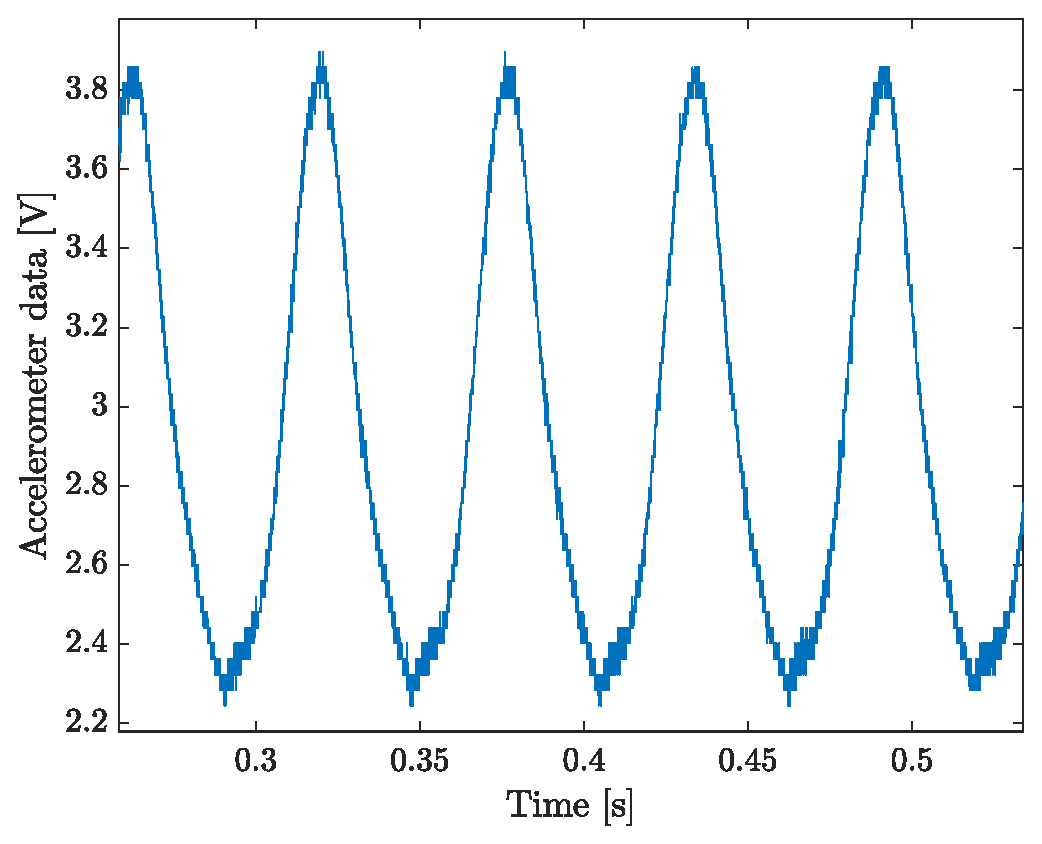
\includegraphics[width=\textwidth]{noball}
	\caption{Accelerometer data for the loudspeaker without the ball.}
	\label{noball}
\end{subfigure}\hfill
\begin{subfigure}[t]{0.49\textwidth}
	\centering
	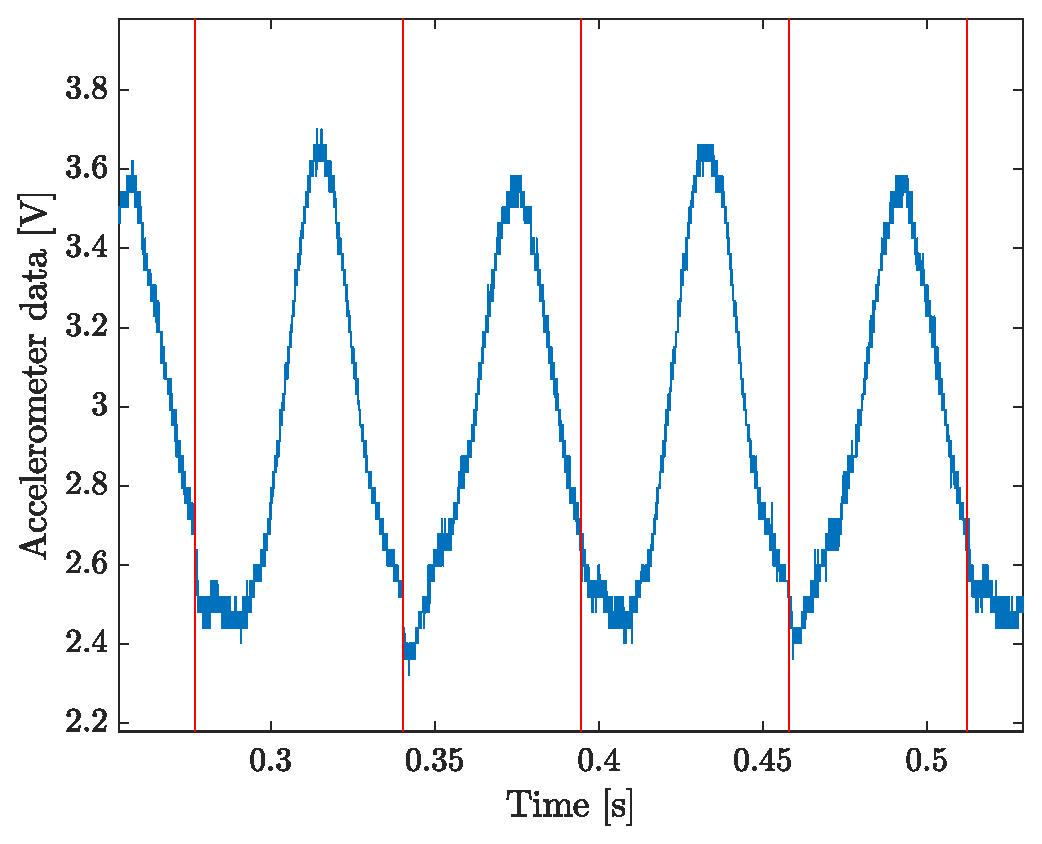
\includegraphics[width=\textwidth]{wball}
	\caption{Accelerometer data for the loudspeaker with the ball in a stable 2 period orbit, the red lines are impacts detected by the piezoelectric element.}
	\label{wball}
\end{subfigure}
\end{figure}
On figure there is a quite noticeable difference in amplitude between the two 
waveforms roughly 20\% less. Also note that the shape of the sine wave on 
figure \ref{wball} is quite off compared to the configuration with no ball. 
This has a quite significant effect on our model since it both assumes the 
amplitude with no ball, a ``nice'' wave form and a perfectly compliant 
loudspeaker. For each impact the acceleration takes a hit, we therefore suggest 
that the velocity of the speaker will be lower than modeled. We also suggest 
that, as the speaker evidently isn't ideal, the speaker will not be able to 
provide the necessary impulse, and in turn, the ball will not have expected 
initial velocity after the collision.
 
\section{Numerical simulation}
\label{Numericalsec}
\subsection{Numerical simulation scheme}
As described in section \ref{modelling} it is not possible to solve the systems 
equations of motion analytically in the general case as it require one to find 
the intersection between a parabola and a sine wave. In the numerical realm it 
is however possible to find this intersection. The actual problem is to find 
where \eqref{membraney} and \eqref{ybeq} are equal that is solving the following
\begin{equation}
	A \cos(2\pi f t+ \phi) = -\frac{g}{2}(t-t_k)^2+v_k(t-t_k)+y_p(t_k)
\end{equation}
As described this can easily be done numerically, and the initial velocity for the next jump follows from the equations derived in section \ref{modelling}. In practice, this is done using the \texttt{fzero} method in \textsc{Matlab}, which is essentially using a bisection method for root finding.

\subsection{Sticky solutions}
For some parameters the trajectory of the ball will end in it sticking to the 
membrane, not bouncing. In our simulation this will be represented as a series 
of zeroes, which can be thought of as the ball bouncing infinitely fast. In 
practice, we have defined a tolerance for our numerical calculations, defined 
as $\SI{1e-5}{\second}$. We will assign a sticky solution to any parameter set 
for which the time between two following jumps is less than this tolerance. 
\subsection{Chaotic behaviour in the theoretical model}
The idea for the experiment originates from Tufillaro and Albano \cite{tufillaro}, who suggested that the bouncing ball behaves very much like the quadratic map described in section \ref{chaos}. This observation seems to hold qualitatively, however the link between the suggested quadratic map and the governing equations of the system seems weak. Nonetheless, simulated data shows behaviour very much analogues to the quadratic map. For some initial conditions, we find there exists stable orbits with period 3, 5 and 7 co-existing with the period 1, 2, 4, and-so-on orbits. While these odd numbered orbits also exists in the quadratic map, they only appear momentarily inside ``islands'' of stability in the chaotic region. The logistic map is a convenient model to introducing chaotic systems, but it appears it is not sufficient to explain the dynamics of the ball-speaker system. In the appendix we will provide simulated and experimental data showing odd period orbits.

\subsubsection{Dependence on initial conditions}
We found through numerical simulations and practical experience that the systems behaviour strongly varies with different initial conditions. Most intriguingly we found that for some initial energies the system will fall into stable period 3 orbits. This effect was also repeatedly demonstrated in the lab. Through numerical simulation we hoped to gain some insight into the connection between the initial velocities and the tendency to drop into period 3 orbits as opposed to $2^n$-period orbits. We have plotted the differences in the time series of the last 50 jumps out of 200 jumps total to allow the system to become stable, for varying values of initial velocity. 
\begin{figure}[h]
\centering
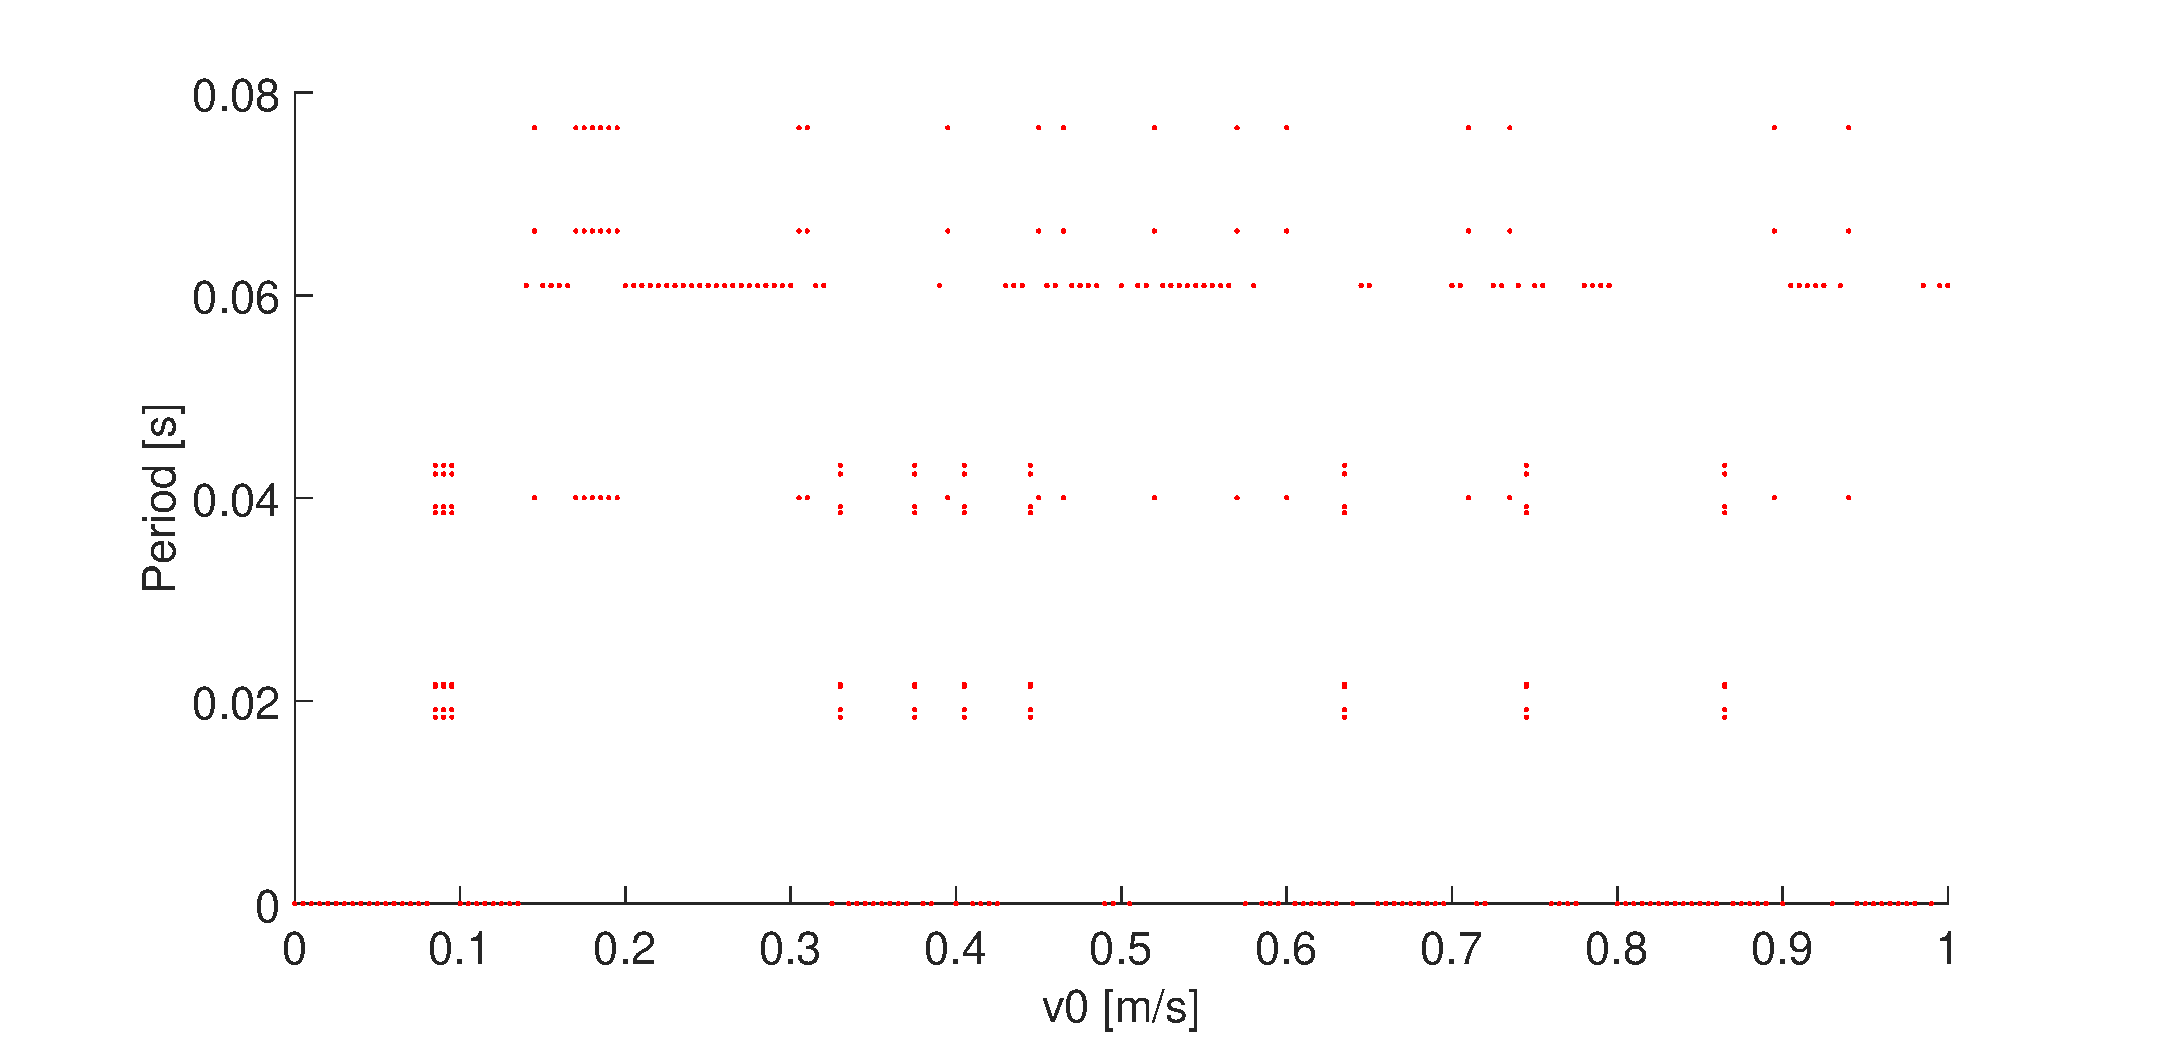
\includegraphics[width=0.65\textwidth]{vsweep.eps}
\caption{Stable solution depends strongly on initial velocity. The system plotted here is simulated with $C_r=0.66$, $f=\SI{16}{Hz}$, $A=\SI{1.1}{mm}$.}
\end{figure}
We cannot claim to identify any strong patterns in this, but we have found that if we limit the initial velocity such that the ball does not skip a period, the simulations appear to be more stable. When simulating our experiment we sweep a range of frequencies, and for each value we start the ball at the top of the waveform with some initial velocity given by:
\begin{align*}
v_0(f) &= \frac{g}{2f} c
\end{align*}
This corresponds to some fraction $c$ of the speed required to jump a whole period of the loudspeaker, which for $0.7<c<0.9$ seems to land the system in the period-doubling, logistic map-esque, attractor. For the simulation plotted, we see there is an island of stable initial velocities in the range $\SI{0.1}{\meter\per\second}$ to $\SI{0.3}{\meter\per\second}$.
\subsection{Measuring Feigenbaums $\delta$}
Using \eqref{Feigenbaumsdelta} we can calculate Feigenbaums constant using the dynamics of our system. Marking the times of the bifurcations in figure  \ref{feigsim}, we can calculate the $\delta$.
\begin{figure}[h]
\centering
\includegraphics[width=0.65\linewidth]{feigplot} 
\caption{Simulated data: $A=\SI{1}{\mm}$ and $C_r=\num{0.6}$ for 500 consecutive jumps, with the last 150 plotted for each frequency. The blue lines matching bifurcations correspond to the frequencies $f=\{\SI{18.1028}{\hertz},\SI{19.0153}{\hertz},\SI{19.1952}{\hertz},\SI{19.2337}{\hertz} \}$.}\label{feigsim}
\end{figure}
The two first values in the series for Feigenbaums $\delta$ for our simulation is:
\begin{align}
\delta&=\frac{\lambda_{n-2} - \lambda_{n-1}}{\lambda_{n-1}-\lambda_n}\\
\delta_1&=\frac{\SI{18.1028}{\hertz}-\SI{19.0153}{\hertz}}{\SI{19.0153}{\hertz}-\SI{19.1952}{\hertz}} = \num{5.1(3)}\\
\delta_2&=\frac{\SI{19.0153}{\hertz}-\SI{19.1952}{\hertz}}{\SI{19.1952}{\hertz}-\SI{19.2337}{\hertz}} = \num{5(1)}
\end{align}
The frequency resolution used here is $\SI{0.0064}{\hertz}$. The uncertainties are calculated with the law of error propagation, where the error is the size of the frequency steps. We can not be sure where the bifurcations are, but using the whole distance, we are sure to cover it.  
\section{Data analysis}
\subsection{Comparison to simulated data}
To see how well our model holds, we can plot the simulated data, and the measured data, which can be seen on figures \ref{realdata} and \ref{fakedata}. Figure \ref{realdata} is a plot of the measured data and simulation with the correct amplitude and $C_r$.
\begin{figure}
\centering
\begin{subfigure}[t]{0.49\textwidth}
	\centering
	\includegraphics[width=\textwidth]{realvals}
	\caption{Measured data in blue, and simulated data in red. The simulation is run with the same parameters as we have set-up the experiment with, and with measured $C_r$.}
	\label{realdata}
\end{subfigure}\hfill
\begin{subfigure}[t]{0.49\textwidth}
	\centering
	\includegraphics[width=\textwidth]{fakevals}
	\caption{Measured data in blue, and simulated data in red. The simulation is run with 83\% of the amplitude, and with the same $C_r$ as measured.}
	\label{fakedata}
\end{subfigure}
\end{figure}
Quite obviously the bifurcations are neither wide nor short enough, which we 
suspect has to do with the ball interacting with the loudspeaker. Because we 
have measured that the actual amplitude is lower as described in section 
\ref{ballmembrane}, we tried with a lower amplitude which resulted in figure 
\ref{fakedata}. Further discussion on this effect will be given in section 
\ref{conclusions}.

\subsection{Feigenbaums $\delta$}
Running the experiment as described in section \ref{expsetup}, we have produced a bifurcation diagram showing three bifurcations. From these, we calculated Feigenbaums $\delta$ using the same methods we used in section \ref{Numericalsec} on the simulated data shown on figure \ref{expfeigplot}.
\begin{figure}[h]
\centering
\begin{subfigure}[t]{0.49\textwidth}
\centering
\includegraphics[width=\textwidth]{feigplotexp}
\caption{Experimental data in blue, lines in red marking the bifurcations.}
\label{expfeigplot}
\end{subfigure} \hfill
\begin{subfigure}[t]{0.49\textwidth}
\centering
\includegraphics[width=\textwidth]{long}
\caption{A run with a smaller and lighter ball. The distance between the first and the second bifurcation is much longer.}
\label{long}
\end{subfigure}
\end{figure}
We find Feigenbaums $\delta$ to be:
\begin{align}
\delta &= \frac{\SI{18.4980}{Hz}-\SI{18.2475}{Hz}}{\SI{18.2475}{Hz}-\SI{18.5707}{Hz}} = \num{3.4(5)}
\end{align}
This number is quite close to Feigenbaums $\delta$, but does not fall inside the uncertainty. Further discussion will be given in the following section.  

\section{Discussion and conclusions}
\label{conclusions}
Our simulated data disagrees strongly with our measured data. We have identified some effects which we have not included in our model. The first is the fact that $C_r$ has some velocity dependence. In Müller et. al. \cite{muller}, they show this effect to be small (roughly 0.5\% drop in the range $\SI{0.3}{\meter\per\second}$ to $\SI{0.7}{\meter\per\second}$) in the velocity range we are using. Second we assume the speaker is perfectly sinusoidal. This proved to be incorrect in the $\SI{14}{Hz}$ to $\SI{16}{Hz}$ range, but less of a issue in the range used. Our main culprit seems to be the backeffect from the ball hitting the speaker. Late in the project we tried to repeat the experiment using a lighter ball, figure \ref{long}. We discovered that this seemed to produce results more like our simulations. We have shown the ring-out of the speaker to be slow, and we have seen that for a period 2 orbit, there is a strong disturbance of the waveform when the ball is bouncing. Future work could be to model the speaker and the effect of the collisions more accurately. We saw the if we reduced the amplitude in our simulations by roughly 20\%, as was the reduction in amplitude produced by the steel ball, we match up the first bifurcation. The spread and the length of the bifurcations, we can however not explain only trough this effect, so this fact seem to be quite incidental. It should be noted that the simulation fits quite well into Feigenbaums theory as it gave a correct $\delta$.
	
The uncertainties in the measurement of Feigenbaums $\delta$ are quite large. The error is our ability to resolve frequencies. In the simulated experiment, this is a case of more computing needed, but in the experimental runs we are limited by our set-ups ability frequency resolution. The fact that we only see three bifurcations makes the measurement especially weak, and limits our ability to confirm the universality of Feigenbaums constant. Though our experiment suggest a reasonable $\delta$ which is approximately the same as seen in Tufillaro and Albano \cite{tufillaro}.
\newpage
\pagenumbering{gobble}

\addcontentsline{toc}{section}{References}
\bibliographystyle{plain}
\bibliography{ref}

% % % % % % % % % % % % % % % % % % % % % % Appendix % % % % % % % % % % % % % % % % % % % % % % % % %
\newpage
\appendix

\pagenumbering{roman}
\setcounter{page}{1}


\section{Cobweb diagrams}
\label{cobwebapen}
\begin{figure}[h]
	\centering
	\begin{subfigure}[t]{0.45\textwidth}
		\centering
		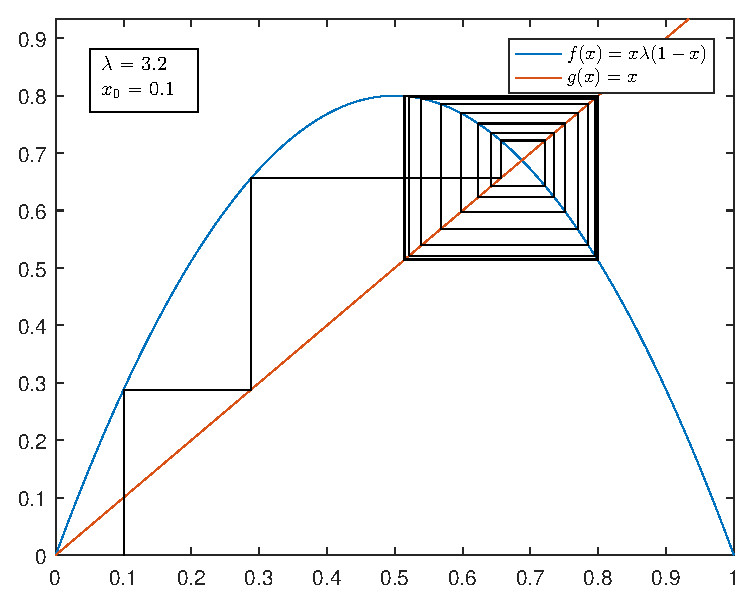
\includegraphics[width=\linewidth]{{Figures/cobweb_x1_l32_iter100}}
		\caption{A stable 2-period}
	\end{subfigure}\hfill
	\begin{subfigure}[t]{0.45\textwidth}
		\centering
		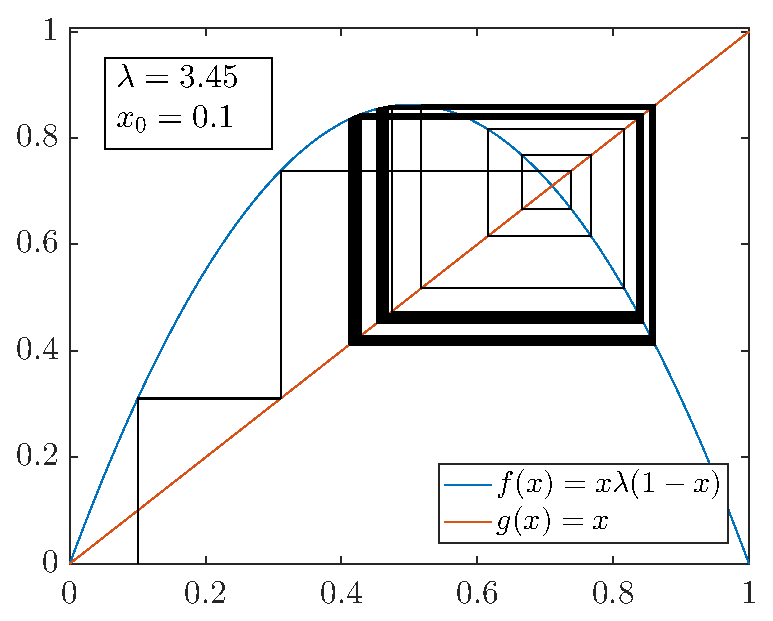
\includegraphics[width=\linewidth]{{Figures/cobweb_x1_l35_iter100}}
		\caption{A stable 4-period}
	\end{subfigure}
\end{figure}

\begin{figure}[h]
	\centering
	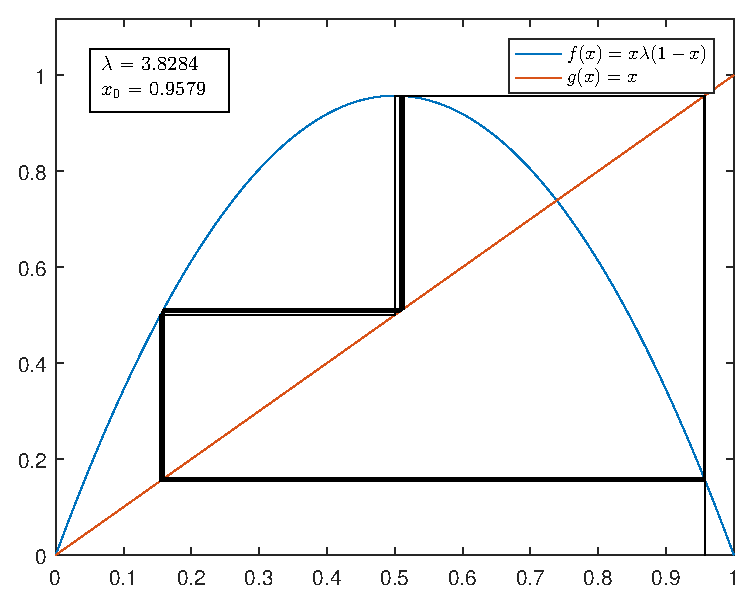
\includegraphics[width=0.65\linewidth]{Figures/cobweb_x10_l38_iter100}
	\caption{Cobweb diagram with $\lambda$ corresponding to a 3-period. The 
	initial condition is chosen to be very close to a value contained in the 
	attractor, since not doing this will create a lot of noise as $x_n$ finds 
	the stable 3-period, which makes it hard to distinguish this diagram from 
	one in the chaotic regime.}
\end{figure}
\newpage
\section{Derivation of the equations of motion for a driven harmonic oscillator}
\label{driven}
The equation of motion for a driven simple harmonic oscillator will be of the form:
\begin{align*}
my'' + by' + ky = F\sin(\omega t)\\
y'' + \frac{b}{m}y' + \frac{k}{m} y = F \sin(\omega t)
\end{align*}
We will then write the general solution as a sum of the particular and the homogeneous solutions:
\begin{align*}
y_g = y_{h} + y_p
\end{align*}
The homogeneous solution for the damped harmonic oscillator will go to zero with time. We claim it is only the particular solution that matters. To solve this, we will guess the solution to be of the form:
\begin{align*}
y_p = A \sin (\omega t) + B \cos(\omega t)
\end{align*}
We will perform the differentiation and plug into the equation to get:
\begin{align*}
&m\left(-A\omega^2\sin(\omega t) - B\omega^2\cos(\omega t)\right) + b\left(A\omega\cos(\omega t) - B\omega\sin(\omega t)\right) + k\left( A\sin(\omega t) + B\cos(\omega t) \right)\\
&=\sin(\omega t) \left( -mA\omega^2 -bB\omega + kA \right) + \cos(\omega t)\left(-mB\omega^2 + bA\omega + Bk\right)
\end{align*}
After collecting the coefficients, we can match the left side, with the right side:
\begin{align}
F &= -mA\omega^2 -bB\omega + Ak \label{lignA} \\ 
0 &= -mB\omega^2 + bA\omega + Bk \label{lignB}
\end{align}
We isolate an expression for $B$ in (\ref{lignB})
\begin{align*}
B &= \frac{-bA\omega}{-m\omega^2+k}
\end{align*}
Which we will proceed to plug into (\ref{lignA}), to obtain an expression for $A$:
\begin{align*}
A = \frac{F}{-m\omega^2+k+\frac{b^2\omega^2}{-m\omega^2+k}} = \frac{F\left(k-m\omega^2\right)}{\left(k-m\omega^2\right)^2+b^2\omega^2}
\end{align*} 
We can write $A$ and $B$ independently of each other:
\begin{align*}
B &= \frac{-bF\omega}{\left(k-m\omega^2\right)^2+b^2\omega^2}\\
A &=  \frac{F\left(k-m\omega^2\right)}{\left(k-m\omega^2\right)^2+b^2\omega^2}
\end{align*}
We would now like to express $y_p$ in the shape:
\begin{align*}
y_p = L \sin(\omega t + \phi)
\end{align*}
If we write the sine addition identity,
\begin{align*}
L sin(\omega t + \phi) = L\cos(\phi)\sin(\omega t) + L\sin(\phi)\cos(\omega t)
\end{align*}
We see, that our amplitude must obey,
\begin{align*}
A = L\cos(\phi)\\
B = L\sin(\phi)
\end{align*}
if we are to get our initial guess of
\begin{align*}
y_p = A \sin (\omega t) + B \cos(\omega t)
\end{align*}
The phase shift will then be:
\begin{align*}
\frac{B}{A} &= \frac{L\sin(\phi)}{L\cos(\phi)} = \tan(\phi)\\
\phi &= \arctan\left(\frac{B}{A}\right)\\
\phi &= \arctan\left( \frac{-bF\omega}{\left(k-m\omega^2\right)^2+b^2\omega^2} \cdot \frac{\left(k-m\omega^2\right)^2+b^2\omega^2}{F\left(k-m\omega^2\right)} \right)\\
\phi &= \arctan\left( \frac{b\omega}{m\omega^2-k} 
\right)=\arctan\left(\frac{2\pi \frac{b}{m} f}{4\pi^2 
	f^2-\frac{k}{m}}\right)
\end{align*}

If our system also has a latent phase shift due to some constant delay in time, such as time lost to processing in the microcontrollers or anywhere else before the signal gets to the loudspeaker, we can simply add this phase shift to our expected phase shift of a driven oscillator.
\begin{equation}
    \phi = \arctan\left(\frac{2\pi \frac{b}{m} f}{4\pi^2 
    f^2-\frac{k}{m}}\right)+\phi_{latent} =\arctan\left(\frac{2\pi \frac{b}{m} 
    f}{4\pi^2 f^2-\frac{k}{m}}\right) + 2\pi f t
    \label{pshifteq}
\end{equation}
We use this equation to model the phaseshift in our loudspeaker, since it seems 
reasonable to suggest that there will be some delay in the signal on its way to 
the loudspeaker.
\newpage
\section{Odd-numbered orbits}



\begin{figure}[h]
	\centering
	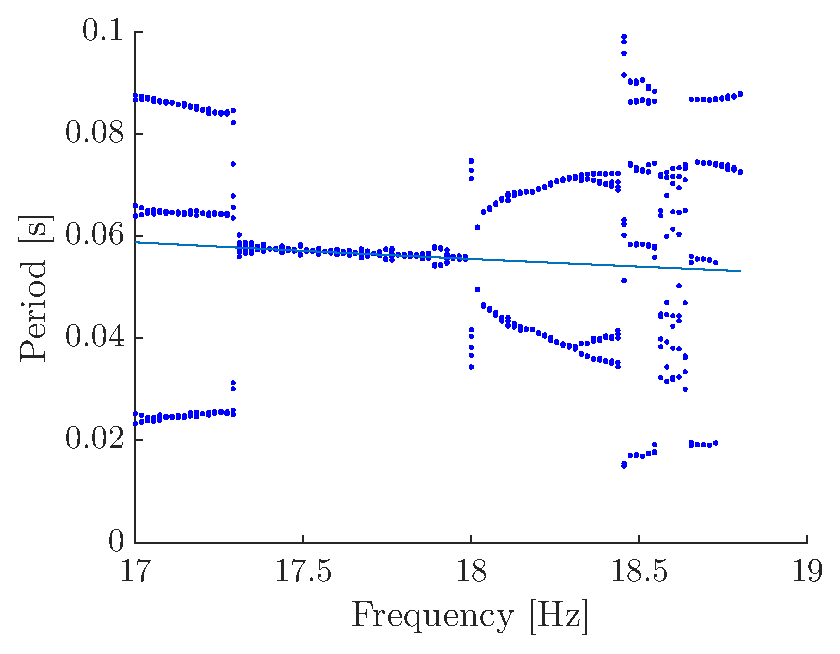
\includegraphics[width=0.65\linewidth]{period3.eps}
	\caption{Odd numbered orbits in experimental data. The light blue line 
		behind the data is a plot of $1/f$, signifying one period of the 
		loudspeaker.}
\end{figure}


\begin{figure}[h]
	\centering
	\includegraphics[width=0.65\linewidth]{3psim.eps}
	\caption{Odd numbered orbits in simulated data.}
\end{figure}

%\begin{figure}[h]
%	\centering
%	\begin{subfigure}[t]{0.45\textwidth}
%		\centering
%	    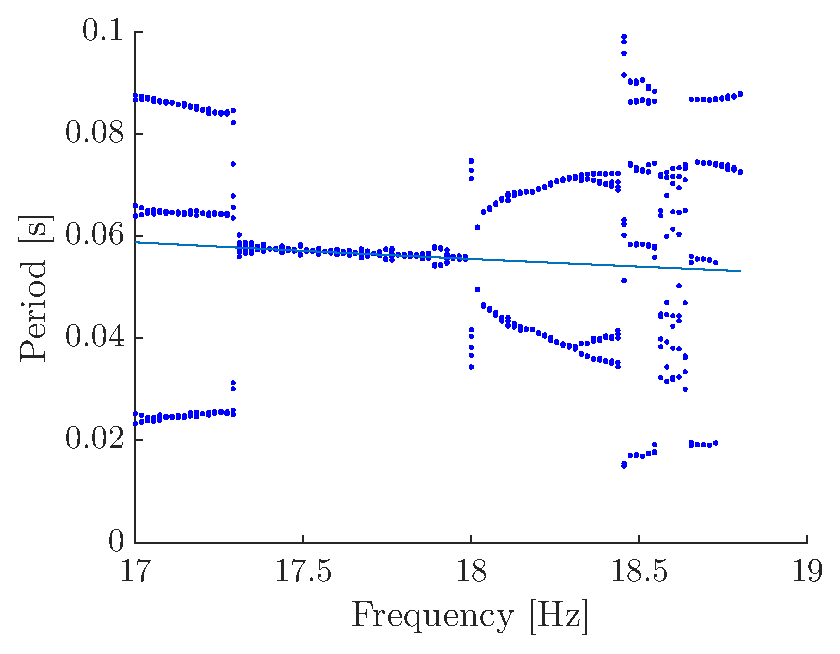
\includegraphics[width=\linewidth]{period3.eps}
%	    \caption{Odd numbered orbits in experimental data. The light blue line 
%	    behind the data is a plot of $1/f$, signifying one period of the 
%	    loudspeaker.}
%	\end{subfigure}\hfill
%	\begin{subfigure}[t]{0.45\textwidth}
%		\centering
%	    \includegraphics[width=\linewidth]{3psim.eps}
%	    \caption{Odd numbered orbits in simulated data.}
%	\end{subfigure}
%\end{figure}
\end{document}